\newpage
\section{Измерения}
Одними из наиболее важных подзадач в рамках любой оптимизационной деятельности являются измерение,
трактовка результатов и определение наиболее важных для оптимизации мест.

В рамках данной главы будут изложены основные подходы, используемые при измерениях, результаты
измерений и их анализ.

\subsection{Корректность}
Измерение производительности программ следует производить с особой осторожностью, так как существует
множество различных факторов, в том числе случайных, влияющих на время их работы.

В случае программы для платформы Java, время ее работы во многом зависит от специфики работы
виртуальной машины.
В частности, изучая результаты измерений, следует уточнять:
\begin{itemize}
    \item Достаточно ли времени было у виртуальной машины для того, чтобы скомпилировать наиболее
    <<горячий>> код.

    Чаще всего непосредственно перед замером код бенчмарка запускается некоторое число раз с целью
    <<разогрева>> виртуальной машины.

    Это нужно не только для того, чтобы дать JVM возможность в принципе скомпилировать код, но и
    для накопления достаточного количества информации о профиле программы, чтобы адаптировать
    скомпилированный код для наиболее частых вариантов исполнения, в т.ч. для удачного расположения
    различных процедур в памяти.

    \item Насколько интенсивно запускаемый код аллоцирует динамическую память, достаточно ли ее.

    В случае жестких ограничений на память существенное время работы программы будет потрачено
    на сборку мусора, которая в особых случаях блокирует поток исполнения.

    \item Могла ли виртуальная машина доказать избыточность той части кода, которая подлежит
    измерению, и удалить соответствущие вычисления.

    В случае наличия такой возможности не может быть и речи о корректности измерений.
\end{itemize}

Для преодоления вышеописанных проблем все бенчмарки, описанные в данной работе, были реализованы
с помощью \textit{JMH}\fu{http://openjdk.java.net/projects/code-tools/jmh/}
--- каркаса для бенчмарков, разрабатываемого инженерами компании Oracle.

Каждый бенчмарк  представляет собой метод, отмеченный аннотацией ``Benchmark'', либо с пустым
набором параметров, либо принимающий объект класса ``Blackhole''.

Измерения производительности бенчмарка состоят из регулируемого числа итераций.
В рамках отдельной итерации код бенчмарка запускается несколько раз примерно в течение секунды,
после чего время работы вычисляется как среднее.

Результаты всех итераций рассматриваются, как выборка из нормального распределения с неизвестной
дисперсией, на основе которой вычисляется мат. ожидание, СКО, и доверительный интервал.

JMH предоставляет авторам бенчмарков ряд возможностей для контроля корректности измерений.
\begin{itemize}
    \item Пользователь может устанавливать число итераций разгогрева для каждого бенчмарка.
    Достаточность этого значения можно определить на основе анализа журнала компиляции HotSpot,
    который можно получить, запустив JVM с опцией ``-XX:+LogCompilation''.

    \item С помощью аннотации ``CompilerControl'' можно устанавливать будет ли конкретный метод
    скомпилирован или встроен JIT-компилятором, что позволяет моделировать различные варианты
    его поведения.

    \item JMH гарантирует, что если некоторое значение возвращено методом-бенчмарком или оно
    передано в качестве аргумента методу ``consume'' объекта ``Blackhole'', то виртуальная машина
    не сможет доказать избыточность кода, влияющего на это значение.

    \item В новых версиях JMH появилась возможность находить участки кода, которые исполняются
    дольше всего в процессе измерений.
    Вычисление наиболее <<горячих>> точек происходит с помощью инструмента ``perf''\fu{http://en.wikipedia.org/wiki/Perf_(Linux)},
    доступного для ОС Linux.

    Вывод результатов производится вместе с машинным кодом соответствующих участков на языке
    ассемблера.
    Это позволяет более точно оценить вклад тех или иных инструкций байт-кода в общее время работы
    бенчмарка.
\end{itemize}

\subsection{Условия проведения измерений}
\begin{itemize}
    \item \textbf{Модель ЦПУ:} Intel(R) Core(TM) i7-3540M CPU @ 3.00GHz
    \item \textbf{Операционная система:} Linux 3.11-2-amd64 \#1 SMP Debian 3.11.8-1 (2013-11-13) x86\_64 GNU/Linux
    \item \textbf{Реализация JVM:} Oracle Hotspot
    \item \textbf{Версии Java Runtime Edition:} 1.6.0\_45, 1.7.0\_51, 1.8.0
    \item \textbf{Ключи JVM:} -Xmx1024M -XX:+AggressiveOpt -XX:+DoEscapeAnalysis
\end{itemize}

\subsection{Бенчмарки}
В данном разделе представлено описание реализованных в рамках данной работы бенчмарков, указано
время их работы и проведен анализ недостатков в сгенерированном байт-коде.

Так как абсолютное время работы бенчмарка само по себе по сути не имеет смысла, для каждого из
них создан в некотом роде семантически эквивалетный эталон, производительность которого
с точки зрения автора должна быть близким к оригиналу.

Например при измерениях, нацеленных на проверку простых синтаксических конструкций, таким эталоном
может служить аналогичный код на Java, а при измерении времени работы стандартных функций высшего
порядка их код с заменой вызовов функционального аргумента на тело анонимной функции.

\subsubsection{АВЛ-дерево}
Одним из бенчмарков с существенно нетривиальным кодом стала реализация АВЛ-дерева, используемая
для решения задачи \textit{Stars}\fu{http://acm.timus.ru/problem.aspx?num=1028&locale=ru}.

По сути решение задачи сводится к последовательному добавлению элементов в дерево с запросом
порядкового номера добавленного элемента в отсортированном множестве.

В качестве <<идеального>> решения была использована реализация АВЛ-дерева, написанная автором
на Java, из которой с использованием автоматической конвертации была получена версия на Kotlin.

Большая часть полученного кода состоит из синтаксических конструкций, которые есть в обоих языках,
и единственным важным отличием стало использование в решении на Kotlin специальных операторов:
так называемые <<безопасный вызов>> и ``elvis''-оператор.

Семантика первого в целом имеет сходство с оператором <<точка>> из Java, но с дополнительной
проверкой выражения на котором происходит вызов на равенство ``null''.
\begin{pyglist}[language=kotlin]
x?.foo() // Safe-call
if (x != null) x.foo() else null
\end{pyglist}
В приведенном участке кода первая строка является примером безопасного вызова, а вторая
выражает его смысл.

Оператор ``elvis'' имеет семантику значения по умолчанию:
\begin{pyglist}[language=kotlin]
nullableInt ?: 0 // elvis
if (nullableInt != null) nullableInt else 0
\end{pyglist}

На практике нередко встречается их совместное использование.
Например при балансировке АВЛ-поддерева необходимо вычислить высоты каждого из двух поддеревьев,
причем при отсутствии поддерева его высота полагается равной нулю.
С помощью описанных выше конструкций высоту например левого поддерева можно выразить следующим
образом:
\begin{pyglist}[language=kotlin]
leftChild?.height ?: 0
\end{pyglist}

\paragraph{Результаты измерений}
Результаты измерений представлены в таблице ниже.
Параметр ``size'' --- количество добавляемых элементов, сами элементы --- случайные точки
на плоскости, но одинаковые в рамках каждого запуска.

\begin{table}[h]
\begin{center}
\begin{tabular}{|c|c|c|c|} \hline
Размер & Java & Kotlin & Фактор \\ \hline
100 & 19.412 $\pm$ 0.266 мкс & 30.687 $\pm$ 1.66 мкс & 1.581\\ \hline
1000 & 300.055 $\pm$ 2.397 мкс & 476.807 $\pm$ 4.243 мкс & 1.589\\ \hline
100000 & 78.686 $\pm$ 3.14 мс & 132.768 $\pm$ 3.938 мс & 1.687\\ \hline
\end{tabular}
\caption{Результаты бенчмарка <<АВЛ-дерево>>}
\end{center}
\end{table}

Из результатов измерений следует, что версия на Kotlin работает примерно в $1.7$ раз хуже, чем
аналогичный код на Java.
После анализа байт-кода обоих версий было сделано предположение, что наибольший вклад в ухудшение
производительности вносит именно вышеупомянутое сочетание операторов.
Для подтверждения гипотезы была релизована еще одна версия на Kotlin, в которой вместо
безопасного вызова и elvis-оператора используется обычный условный оператор вида:
\begin{pyglist}[language=kotlin]
if (leftChild != null) leftChild.height else 0
\end{pyglist}

Результаты модифицированной версии бенчмарка:

\begin{table}[h]
\begin{center}
\begin{tabular}{|c|c|c|c|} \hline
Размер & Java & Kotlin & Фактор \\ \hline
100 & 19.412 $\pm$ 0.266 мкс & 23.801 $\pm$ 0.367 мкс & 1.226\\ \hline
1000 & 300.055 $\pm$ 2.397 мкс & 331.832 $\pm$ 2.14 мкс & 1.106\\ \hline
100000 & 78.686 $\pm$ 3.14 мс & 87.722 $\pm$ 4.974 мс & 1.115\\ \hline
\end{tabular}
\caption{Результаты бенчмарка <<АВЛ-дерево>> (упрощенная версия)}
\end{center}
\end{table}

Такая версия бенчмарка существенно приблизилась в плане производительности к эталону, таким образом
подтвердив предположение.
Это побудило к более тщательному исследованию производительности кода, генерируемого
для этих операторов, результаты которого изложены в следующем разделе.

\subsubsection{Безопасный вызов и elvis-оператор}
Для уточнения производительности вышеописанного сочетания был реализован следующий микро-бенчмарк:
\begin{itemize}
    \item Определен класс ``Data'' с единственным полем, содержащим целое число
    \item Перед запуском создается массив фиксированного размера, который заполняется с некоторой
    вероятностью либо нулевой ссылкой, либо объектом класса ``Data'' со случайным числом.
    \item Код бенчмарка берет последовательно элементы массива, и для каждого из них
    вычисляет выражение:
    \begin{pyglist}[language=kotlin]
    obj?.x ?: 1
    \end{pyglist}
    \item В качестве эталонного бенчмарка вычисляется эквивалентное выражение с помощью простого
    условного оператора:
    \begin{pyglist}[language=kotlin]
    if (obj != null) obj.x else 1
    \end{pyglist}

    \item Вероятность нулевой ссылки меняется с шагом $0.4$ от $0.1$ до $0.9$.
\end{itemize}

\begin{table}[h]
\begin{center}
\begin{tabular}{|c|c|c|c|} \hline
$p$ & Эталон (мкс) & Бенчмарк (мкс) & Фактор \\ \hline
0.1 & 4.693 $\pm$ 0.036 & 9.131 $\pm$ 0.126 & 1.946\\ \hline
0.5 & 7.103 $\pm$ 0.078 & 7.138 $\pm$ 0.263 & 1.005\\ \hline
0.9 & 4.561 $\pm$ 0.043 & 4.738 $\pm$ 0.047 & 1.039\\ \hline
\end{tabular}
\caption{Результаты бенчмарка "Безопасный вызов и elvis" \newline (p --- вероятность нулевой ссылки)}
\end{center}
\end{table}

Из результатов можно сделать следующие выводы:
\begin{itemize}
    \item Для сочетания операторов безопасного вызова и elvis действительно генерируется байт-код
    уступающий в производительности байт-коду семантически аналогичного условного выражения.

    \item Так как сильнее всего это проявляется когда большая часть объектов не является нулевыми
    ссылками ($p = 0.1$), проблемное место находится в ветвлении для где `obj` не равен `null`.
\end{itemize}

%\begin{verbatim}
                %aload_1 // Загрузка `obj` на стек     
                %dup         
                %ifnull l1
                %getfield x
                %invokestatic  java/lang/Integer.valueOf() // Боксинг
                %goto          l3
                %l1: pop         
                %aconst_null 
                %// начало кода elvis-оператора
                %l2: dup         
                %ifnull l3
                %invokevirtual java/lang/Number.intValue() // Распаковка
                %goto          l4
                %l3: pop         
                %iconst_1
                %l4: ...
%\end{verbatim}

\begin{figure}
\begin{center}
    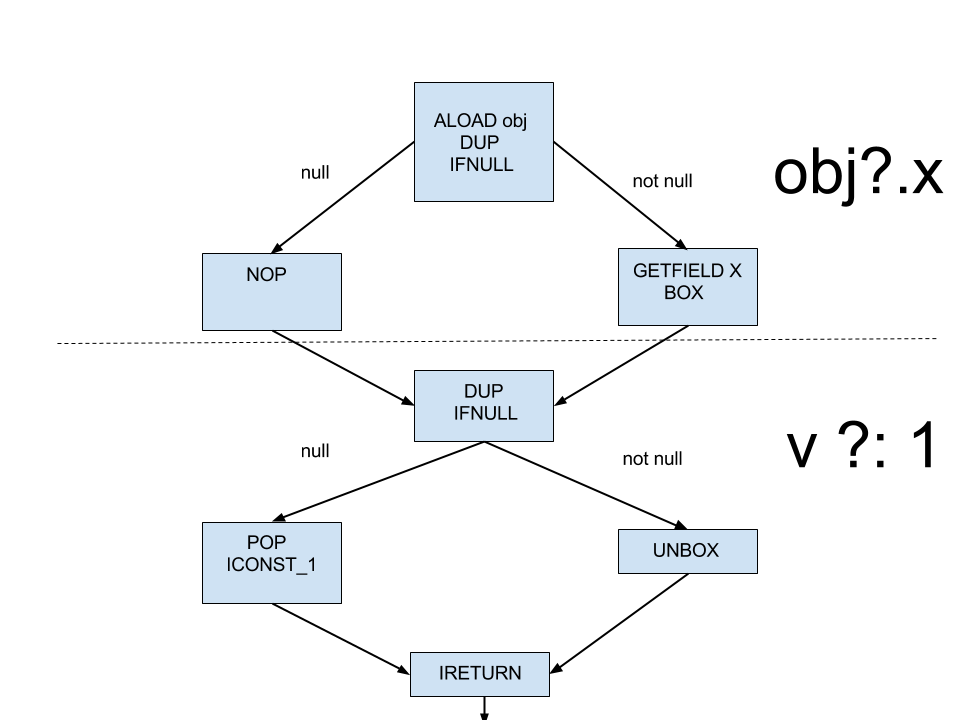
\includegraphics[scale=0.4]{../resources/safecall_elvis.png}
\end{center}
\caption{Блок-схема байт-кода для выражения ``return (obj?.x ?: 1)''}
\label{sc:elvis}
\end{figure}

Примерная блок-схема байт-кода бенчмарка изображена на рисунке \ref{sc:elvis}.
Часть, расположенная выше пунктирной линии описывает генерацию безопасного вызова:
\begin{itemize}
    \item На стек загружается переменная ``obj'', ее значение копируется с помощью инструкции
    ``DUP'', и копия проверяется на равенство ``null''.
    \item В случае если ``obj'' является нулевой ссылкой, то лежащее на вершине стека значение
    тоже нулевая ссылка.
    Иначе на стеке лежит объект ``obj'', у которого берется значение в поле ``x'' и упаковывается.
\end{itemize}

Таким образом обеспечивается контракт безопасного вызова, и на вершине стека находится либо нулевая
ссылка, либо упакованное значение поля.

Боксинг в данном случае необходим, так как ситуация, когда при одном потоке исполнения в ячейке
стека значение примитивного типа, а при другом --- ссылка, запрещена спецификацией виртуальной
машины\cite{JVMSpec}.

Вторая часть блок-схемы иллюстрирует байт-код для elvis-оператора:
\begin{itemize}
    \item Значение, лежащее на вершине стека, копируется и проверяется на равенство нулевой ссылке.
    \item В случае, если оно является нулевой ссылкой, то его копия снимается со стека и
    загружается значение по умолчанию --- целочисленная константа <<1>>.

    Иначе не стеке лежит объект класса ``java.lang.Integer'', из которого и получается значение
    с помощью вызова метода ``intValue'', на блок-схеме этот вызов отмечен для простоты, как
    ``UNBOX''.
\end{itemize}

Понятно, что байт-код этих операторов по отдельности наиболее очевидным образом выражает
их семантику, и выразить их еще проще в рамках спецификации JVM, пожалуй, не представляется
возможным.
Однако их сочетание ни в коей мере оптимальным не кажется.

\begin{figure}
\begin{center}
    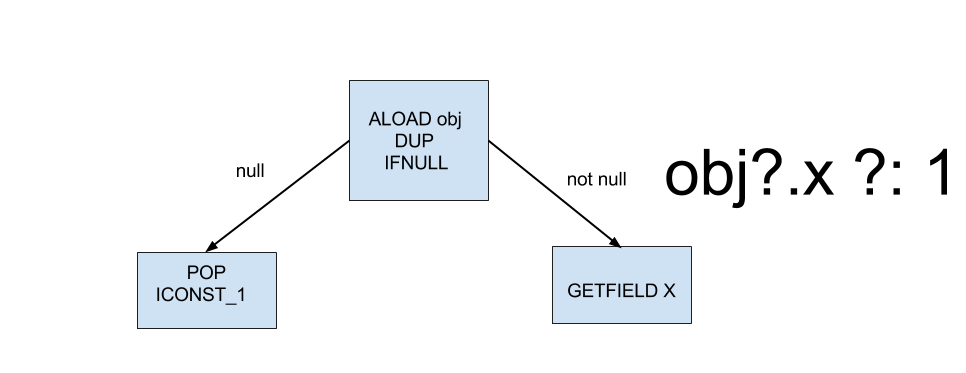
\includegraphics[scale=0.4]{../resources/safecall_elvis_optim.png}
\end{center}
\caption{Блок-схема байт-кода для выражения ``return (obj?.x ?: 1)'' (оптимальный вариант)}
\label{sc:elvisOpt}
\end{figure}

Наиболее кратким вариантом трансляции кажется изображенный на рисунке \ref{sc:elvisOpt}:
\begin{itemize}
    \item Переменная ``obj'' загружется на стек, создается ее копия, и сравнивается с нулевой
    ссылкой.
    \item Если значение является нулевой ссылкой, то его копия снимается со стека, и загружается
    значение по умолчанию.
    Иначе на вершине стека хранится объект, у которого берется значение поля ``x''.
\end{itemize}

При такой генерации отсутствуют операции боксинга, что, как выяснилось в рамках измерений,
хуже всего влияет на производительность вышеописанного байт-кода.

Оптимизации, направленные на решение найденной проблемы, описаны в разделе . % TODO: \ref

\subsubsection{Оператор when}
Оператор ``when'' в Kotlin является в некотором смысле расширением оператора ``switch'' в Java.
Если последний имеет ограниченный набор типов значений, для которых его можно использовать, то
``when'' определен для любых типов, и кроме сравнения на равенство его можно использовать для
проверки принадлежности чисел интервалу, или как некоторую разновидность паттерн-матчинга:

\begin{pyglist}[language=kotlin]
    when(x) {
        1, 2, 3, parseInt(s) -> print(1)
        in 4..1000 -> print(2)
        is String -> print(3)
        else -> print(4)
    }
\end{pyglist}
В случае неконстантных выражений-условий наиболее разумным способом генерации кажется простая
последовательная проверка истинности проверяемых выражений.
При трансляции байт-код для ``when'' аналогичен байт-коду цепочки ``if-else'' операторов,
производительность которых в Kotlin так или иначе не хуже аналогов из Java.

Важно отметить, что оператор ``switch'' можно применять только для набора выражений, которые можно
вычислить во время компиляции.
Причем при трансляции в байт-код используются специальные инструкции \textit{tableswitch} и
\textit{lookupswitch}\cite{JVMSpec}.
Их объединяет общая семантика:
\begin{itemize}
    \item Они параметризуются отображением из набора целых чисел в указатели на другие инструкции
    метода.
    \item При исполнении инструкции интерпретатор снимает с вершины стека число и совершает
    соответствующий переход.
\end{itemize}

Различия заключаются в том, что
\begin{itemize}
    \item \textit{tableswitch} параметризуется интервалом $[high..low]$.
    Для каждого целочисленного значения из этого интервала должна быть задана метка перехода,
    а кроме этого указатель на инструкцию по умолчанию.

    Таким образом размер этой инструкции линейно зависит от ширины интервала.
    \item \textit{lookupswitch} параметризуется отсортированным набором пар значений и меток
    перехода.

    Размер такой инструкции зависит линейно от числа значений.
\end{itemize}

Несмотря на то, что в спецификации не указана трудоемкость выполнения этих инструкций, из формата
их описания понятно, что ``tableswitch'' может быть исполнен за $O(1)$ прямым вычислением индекса
следующей инструкции, а ``lookupswitch'' может быть реализован на основе бинарного поиска и
работать за $O(log\ n)$.

На момент начала данного исследования эти инструкции не использовались в компиляторе Kotlin,
в связи с чем возникла необходимость оценить проигрыш в производительности для случая констант
времени компиляции по сравнению с Java.

Для этого был реализован следующий набор бенчмарков:
\begin{itemize}
    \item Функции с операторами ``switch''/``when'' с набором из последовательных значений
    для сопоставления из интервала $1..20$.
    Каждое условное ветвление представляет из себя оператор ``return'' с уникальным целым числом.
    Предполагается в Java такой ``switch'' транслируется в инструкцию ``tableswitch'',
    предзначначенную как раз для последовательных интервалов.

    \item Бенчмарки, аналогичные предыдущим, но с еще одним условным значением, значительно
    выходящим за пределы интервала $1..20$ --- $0$.
    Предполагается, что здесь должна быть использована инструкция ``lookupswitch'', подходящая
    для разреженных интервалов.

    \item Бенчмарки где операторы ``switch'' и ``when'' применяются для значений класса-перечисления
    (enum).
    Всего в классе объявлено 100 значений, в условном операторе используется 50 с четными номерами.

    \item Бенчмарки, где операторы ``switch'' и ``when'' применяются для строк.
    В качестве выражений для сопоставления использовались строки с вида <<ABCDEFGHIJKLMNO[i]>>,
    где $i$ --- порядковый номер в интервале $1..50$.

    В качестве аргументов использовались случайно выбранные строки из этого же множества.
\end{itemize}

Бенчмарки запускались в цикле на 1000 значений, выбранных случайным образом.

\begin{table}[h]
\begin{center}
\begin{tabular}{|c|c|c|c|} \hline
Разреженность & Java (мкс) & Kotlin (мкс) & Фактор \\ \hline
1..20 & 4.281 $\pm$ 0.018 & 7.8 $\pm$ 0.131 & 1.822\\ \hline
1..20, 100500 & 5.554 $\pm$ 0.077 & 7.524 $\pm$ 0.065 & 1.355\\ \hline
\end{tabular}
\caption{Сравнение производительности операторов switch/when для целочисленных констант}
\end{center}
\end{table}

\begin{table}[h]
\begin{center}
\begin{tabular}{|c|c|c|c|} \hline
Тип & Java (мкс) & Kotlin (мкс) & Фактор \\ \hline
Enum & 10.501 $\pm$ 0.167 & 13.885 $\pm$ 0.037 & 1.322\\ \hline
Строки & 21.667 $\pm$ 0.205 & 81.931 $\pm$ 1.671 & 3.781\\ \hline
\end{tabular}
\caption{Сравнение производительности операторов switch/when для классов перечислений и строк}
\end{center}
\end{table}

Из результатов измерений видно, что разница в производительности различных реализаций
составляет от $1.3$ до $3.7$ раз.

А так как использование константных выражений в подобного рода операторах является довольно
распространенной в программировании практикой, то при генерации следует рассмотреть такой
отдельно и при наличии возможность использовать оптимизирующие инструкции.

Подробности реализации оптимизации для данного случая можно рассмотреть в разделе . %% TODO: \ref

\subsubsection{Встраивание функций}
Изначально предполагается, что производительность встроенных функций должна быть аналогична
производительности кода, полученного при ручном встраивании.

Например код вызова:
\begin{pyglist}[language=kotlin]
    arrayOfInts.count { element -> element > 0 }
\end{pyglist}

где функция ``count'' определена как
\begin{pyglist}[language=kotlin]
    inline fun IntArray.count(predicate: (Int) -> Boolean): Int {
        var count = 0
        for (element in 0..size) {
            if (block(element)) {
                count++
            }
        }
        return count
    }
\end{pyglist}
не должен существенно уступать по производительности коду:
\begin{pyglist}[language=kotlin]
        var count = 0
        for (element in 0..size) {
            if (element > 0) {
                count++
            }
        }
\end{pyglist}

Однако, как было отмечено в разделе \ref{section:scala} добиться этого не слишком просто.

Для проверки влияния встраивания функций на производительность был реализован ряд бенчмарков,
каждый из которых проверяет эффективность различных функций стандартной библиотеки Kotlin
для работы с коллекциями:
\begin{itemize}
    \item ``count'' --- возвращает число элементов коллекции, удовлетворяющих заданному
    предикату-аргументу.
    \item ``filter'' --- возвращает ``ArrayList'' из значений коллекции, удовлетворяющих заданному
    предикату-аргументу.
    \item ``fold'' --- выполняет левоассоциативную свертку элементов коллекции, используя
    в качестве бинарной операции функцию-аргумент.
\end{itemize}

В качестве аргумента для функций использовался целочисленный массив, заполенный случайными числами.
Бенчмарки запускались для размеров массивов: 100, , 00.

В качестве эталонной версии использовался код, встроенный <<вручную>>, как в примере выше.

\begin{table}[h]
\begin{center}
\begin{tabular}{|c|c|c|c|} \hline
Размер & Эталон & Встроенная версия & Фактор \\ \hline
100 & 87.968 $\pm$ 0.78 нс & 348.255 $\pm$ 11.299 нс & 3.959\\ \hline
10000 & 18.401 $\pm$ 0.251 мкс & 78.05 $\pm$ 0.981 мкс & 4.242\\ \hline
1000000 & 3.715 $\pm$ 0.021 мс & 8.565 $\pm$ 0.098 мс & 2.306\\ \hline
\end{tabular}
\caption{Сравнение производительности вызова ``count \{ it \% 2 == 0 \}'' и аналогичного кода, встроенного вручную}
\label{bm:count}
\end{center}
\end{table}

\begin{table}[h]
\begin{center}
\begin{tabular}{|c|c|c|c|} \hline
Размер & Эталон & Встроенная версия & Фактор \\ \hline
100 & 598.23 $\pm$ 5.017 нс & 711.114 $\pm$ 8.057 нс & 1.189\\ \hline
10000 & 98.655 $\pm$ 1.764 мкс & 121.1 $\pm$ 1.74 мкс & 1.228\\ \hline
1000000 & 11.868 $\pm$ 0.529 мс & 13.68 $\pm$ 1.195 мс & 1.153\\ \hline
\end{tabular}
\caption{Сравнение производительности вызова ``filter \{ it \% 2 == 0 \}'' и аналогичного кода, встроенного вручную}
\label{bm:filter}
\end{center}
\end{table}

\begin{table}[h]
\begin{center}
\begin{tabular}{|c|c|c|c|} \hline
Размер & Эталон & Встроенная версия & Фактор \\ \hline
100 & 27.676 $\pm$ 0.159 нс & 477.024 $\pm$ 3.474 нс & 17.236\\ \hline
10000 & 2.784 $\pm$ 0.021 мкс & 47.563 $\pm$ 0.57 мкс & 17.084\\ \hline
1000000 & 301.023 $\pm$ 1.828 мкс & 4.69 $\pm$ 0.031 мс & 15.581\\ \hline
\end{tabular}
\caption{Сравнение производительности вызова ``fold(0) \{ sum, x -> sum + x \}'' и аналогичного кода, встроенного вручную}
\label{bm:fold}
\end{center}
\end{table}

Из результатов (см. таблицы \ref{bm:count}, \ref{bm:filter}, \ref{bm:fold}) видно, что код
встроенных версий от $1.$ до $16$ раз менее производительный, чем в принципе мог бы быть.

При профилировании с помощью плагина ``perfasm'' для JMH было установлено, что наибольший вред
для производительности приносит избыточный боксинг, оставшийся в качестве артефакта от встраивания
параметрически-полиморфного метода ``invoke'' анонимного класса (см. раздел \ref{section:lambda}).
Эта проблема так или иначе уже была поднята в рамках исследования\cite{ScalaDragos} и обсуждена
в рамках раздела \ref{section:scala}.

Наименее всего это влияет на бенчмарк ``filter'', так как значения все равно должны быть запакованы
перед сохранением в ''ArrayList``.

Сильнее всего разница заметна в случае бенчмакр ``fold'', где вычисляется сумма элементов массива.
Это связано с тем, что более чистый байт-код версии, написанной вручную, позволяет компилятору
HotSpot выполнить т.н. размотку цикла, суммирая в каждой итерации по $10$ элементов массива.

Оптимизации, связанные с улучшением производительности встраиваемых функций, описаны в разделе . %% TODO: \ref

\subsubsection{Замена на стеке}
Одной из разновидностей динамической трансляции, реализованной в Hotspot, является так называемая
<<Замена на стеке>> или ``On stack replacement''(OSR), описанная в \cite{HotspotServer}.

В отличие от простой версии JIT-компиляции, когда оптимизированная версия метода используется
только при следующем его вызове, OSR позволяет перейти к исполнению скомпилированного кода в рамках
уже начатого вызова.

Это может быть полезно, например, в случае, когда метод, содержащий цикл с трудоемкими вычислениями,
начал исполняться в режиме интерпретации, и при этом число итераций этого цикла достаточно велико.
В этом случае, если количество итераций преодолело порог-параметр ``OnStackReplaceThreshold'',
код метода компилируется, и в рамках следующей итерации исполняется оптимизированная версия.

Как следует из примера выше, для измерения времени работы необходим бенчмарк, содержащий долго
работающий цикл.
Такими бенчмарками могут послужить описанные в предыдущем разделе при больших размерах массива,
во время анализа работы которых было обнаружено странное поведения при компиляции метода на стеке.

А именно, функция ``foldBenchmark'' вида:
\begin{pyglist}[language=kotlin]
    fun foldBenchmark(): Int {
        return array.fold(0) { (x, y) -> x + y }
    }
\end{pyglist}

за разумное время компилировался <<на стеке>>, и хотя время его работы примерно в 20 раз
отличалось от эталонного, это можно было объснить избыточным боксингом.

Однако байт-код для семантически схожей функции ``foldBenchmarkOSR'' оказался в десятки раз менее
производительным, чем предыдущий (см. таблицы \ref{bm:foldOSR}, \ref{bm:foldOSR2}).
\begin{pyglist}[language=kotlin]
    fun foldBenchmarkOSR(bh: Blackhole) {
        bh.consume(array.fold(0) { (x, y) -> x + y })
    }
\end{pyglist}

Особенно интересным фактом в результатах измерений является то, что производительность второй
версии не уступает обычной версии ``fold'' при малых размерностях.
А кроме того, такое различие наблюдается только при запуске на версиях Hotspot 1.7, 1.8, когда
время на Hotspot 1.6 не отличается (см. таблицу \ref{bm:foldOSR3}).

\begin{table}[h]
\begin{center}
\begin{tabular}{|c|c|c|c|} \hline
Размер & Эталон & foldBenchmarkOSR & Фактор \\ \hline
100 & 27.832 $\pm$ 0.341 нс & 595.958 $\pm$ 4.061 нс & 21.413\\ \hline
10000 & 2.773 $\pm$ 0.006 мкс & 95.095 $\pm$ 0.832 мкс & 34.297\\ \hline
1000000 & 301.701 $\pm$ 4.575 мкс & 114.624 $\pm$ 2.055 мс & 379.925\\ \hline
\end{tabular}
\caption{Сравнение производительности вызова ``foldBenchmarkOSR'' и аналогичного кода, встроенного вручную (версия Hotspot 1.7)}
\label{bm:foldOSR}
\end{center}
\end{table}

\begin{table}[h]
\begin{center}
\begin{tabular}{|c|c|c|c|} \hline
Размер & fold & foldBenchmarkOSR & Фактор \\ \hline
100 & 594.34 $\pm$ 6.472 нс & 595.958 $\pm$ 4.061 нс & 1.003\\ \hline
10000 & 100.181 $\pm$ 0.584 мкс & 95.095 $\pm$ 0.832 мкс & 0.949\\ \hline
1000000 & 11.28 $\pm$ 0.063 мс & 114.624 $\pm$ 2.055 мс & 10.162\\ \hline
\end{tabular}
\caption{Сравнение производительности вызова ``foldBenchmarkOSR'' и аналогичного кода из бенчмарка ``fold'' (версия Hotspot 1.7)}
\label{bm:foldOSR2}
\end{center}
\end{table}

\begin{table}[h]
\begin{center}
\begin{tabular}{|c|c|c|c|} \hline
Размер & fold & foldBenchmarkOSR & Фактор \\ \hline
100 & 477.024 $\pm$ 3.474 нс & 478.739 $\pm$ 5.202 нс & 1.004\\ \hline
10000 & 47.563 $\pm$ 0.57 мкс & 47.482 $\pm$ 0.422 мкс & 0.998\\ \hline
1000000 & 4.69 $\pm$ 0.031 мс & 4.685 $\pm$ 0.051 мс & 0.999\\ \hline
\end{tabular}
\caption{Сравнение производительности вызова ``foldBenchmarkOSR'' и аналогичного кода из бенчмарка ``fold'' (версия Hotspot 1.6)}
\label{bm:foldOSR3}
\end{center}
\end{table}
Причем различия заметны только при больших размерностях задачи, что и дает повод искать корни
проблемы в трансляции <<на стеке>>, так как вероятно метод не успевает запуститься достаточное
число раз для полной компиляции.

После анализа журналов компиляции было определено, что компилятор Hotspot версий 7 и 8
не поддерживает для <<замены на стеке>> циклы, в начале которых стек виртуальной машины не пуст.

\begin{quote}
\begin{verbatim}
<failure reason='OSR starts with non-empty stack'/>
<failure reason='OSR starts with non-empty stack' phase='compile'/>
\end{verbatim}

\captionof{floatquote}{Фрагмент журналов компиляции}
\end{quote}

\begin{verbatim}

\end{verbatim}

Такая ситуация, когда цикл начинается с непустым стеком принципиально невозможна в Java, где
цикл не может быть частью выражения.

Однако проблема может возникнуть в языках, таких как Scala и Kotlin, где любые операторы являются
также и выражениями, то есть пример, описанный ниже --- корректная синтаксическая конструкция:
\begin{pyglist}[language=kotlin]
    fun foldBenchmarkOSR(bh: Blackhole) {
        foo().bar(for (i in 1..100) { print(i) })
    }
\end{pyglist}

Так как результат выражения ``foo()'' должен быть вычислен до выполнения аргумента вызова
``bar()'', то перед началом цикла на вершине стека находится результат ``foo()'', что и приводит
к невозможности проведения замены на стеке.

Несмотря на то, что использование цикла внутри выражения не имеет смысла, аналогичная ситуация
возникает и в разумных случаях, таких как в бенчмарке ``foldBenchmarkOSR'', где перед началом
цикла встроенной функции ``fold'' на стеке загружена переменная ``bh''.

Аналогичная проблема возникает и при встраивании функций в Scala\fu{https://issues.scala-lang.org/browse/SI-8057}.
Оптимизации, связанный с найденной проблемой описаны в разделе . %% TODO: \ref
